% =============================================================================
\section{Introduction}
\emph{Jungle Rest Stop} is a real-time 3D scene made with OpenGL 3.3: a rest stop with a lounge, an ATM room
and a library in a jungle clearing. The user walks around and operates the vending machines, the ATM and the
coffee machine, while visitors arrive by car and use them too. Every object is built only from basic shapes
placed with translation, rotation and scaling; no model or image files are loaded.

% =============================================================================
\section{Overview of the Scene}\label{sec:tour}
\newcommand{\IntroW}{0.97}
\begin{figure}[H]\centering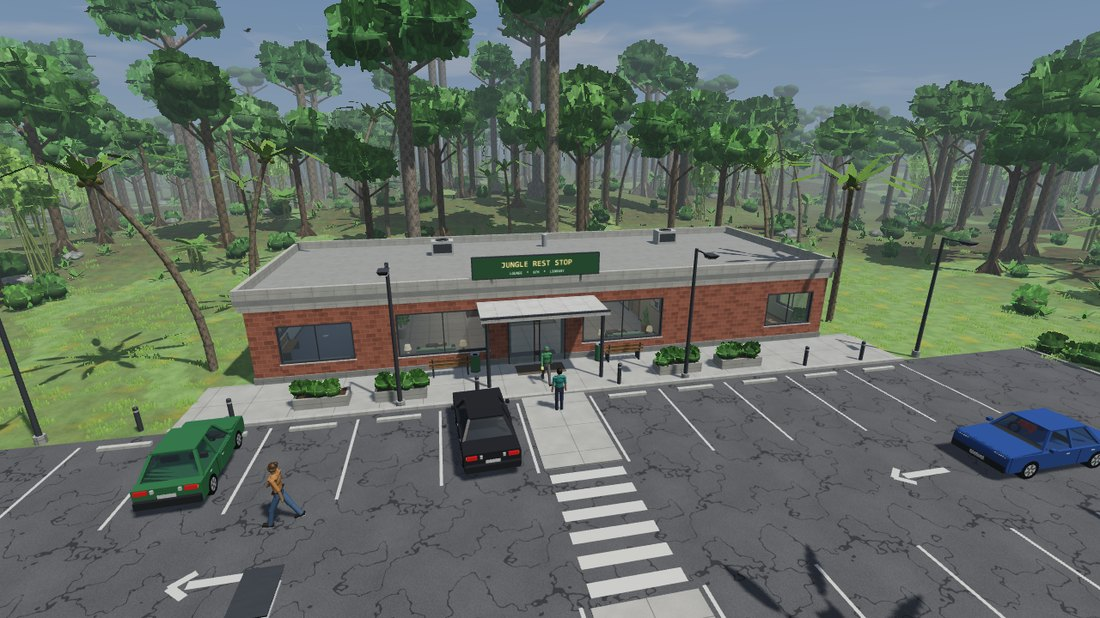
\includegraphics[width=\IntroW\linewidth]{ext_day}\caption{The rest stop by day: building, sidewalk, parking lot and street lamps.}\label{fig:extday}\end{figure}
\shot[\IntroW]{tour_lounge}{The main lounge: sofas, TV wall, coffee counter and the three vending machines.}
\shot[0.86]{tour_vending}{The three vending machines: cold drinks, crispy snacks and sweet treats.}
\begin{figure}[H]
\centering
\begin{subfigure}{0.49\linewidth}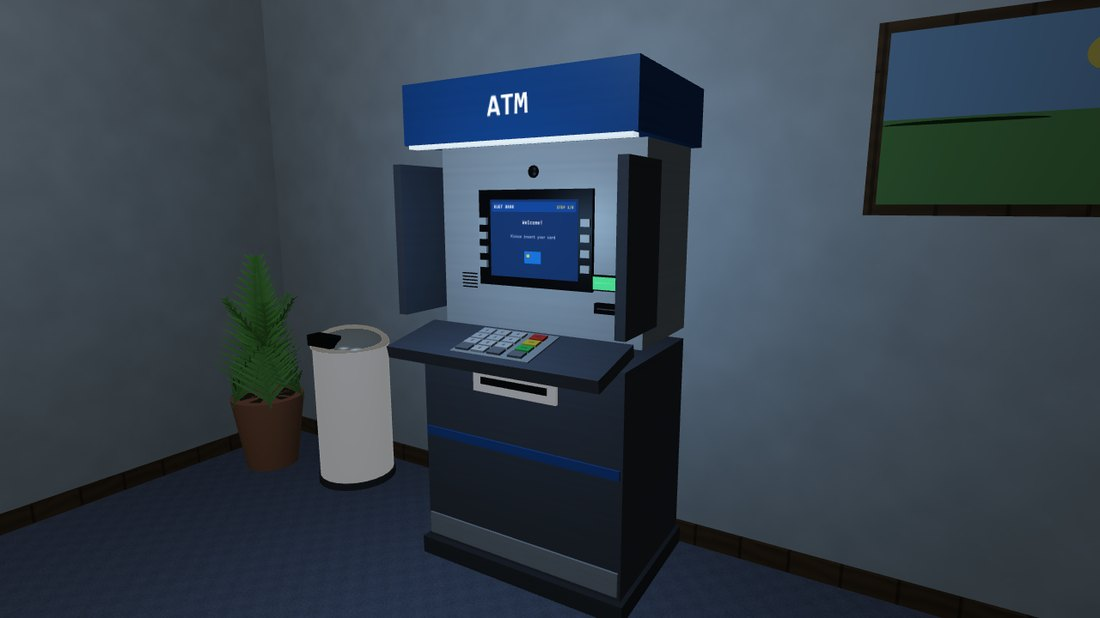
\includegraphics[width=\linewidth]{tour_atm}\caption{ATM room}\end{subfigure}
\begin{subfigure}{0.49\linewidth}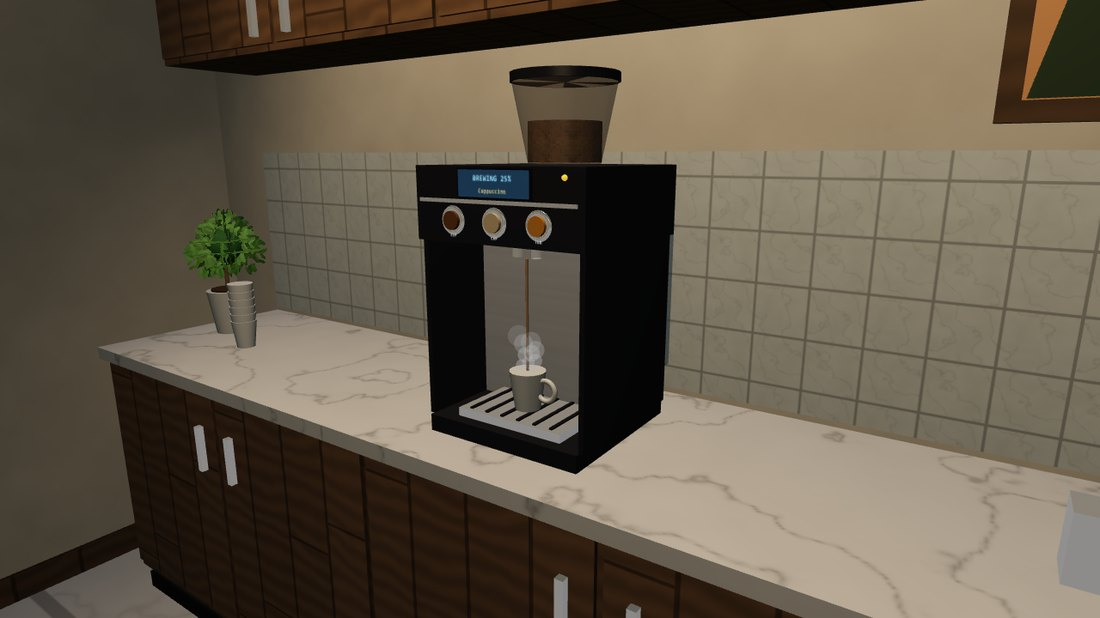
\includegraphics[width=\linewidth]{tour_coffee}\caption{Coffee machine (brewing)}\end{subfigure}
\begin{subfigure}{0.49\linewidth}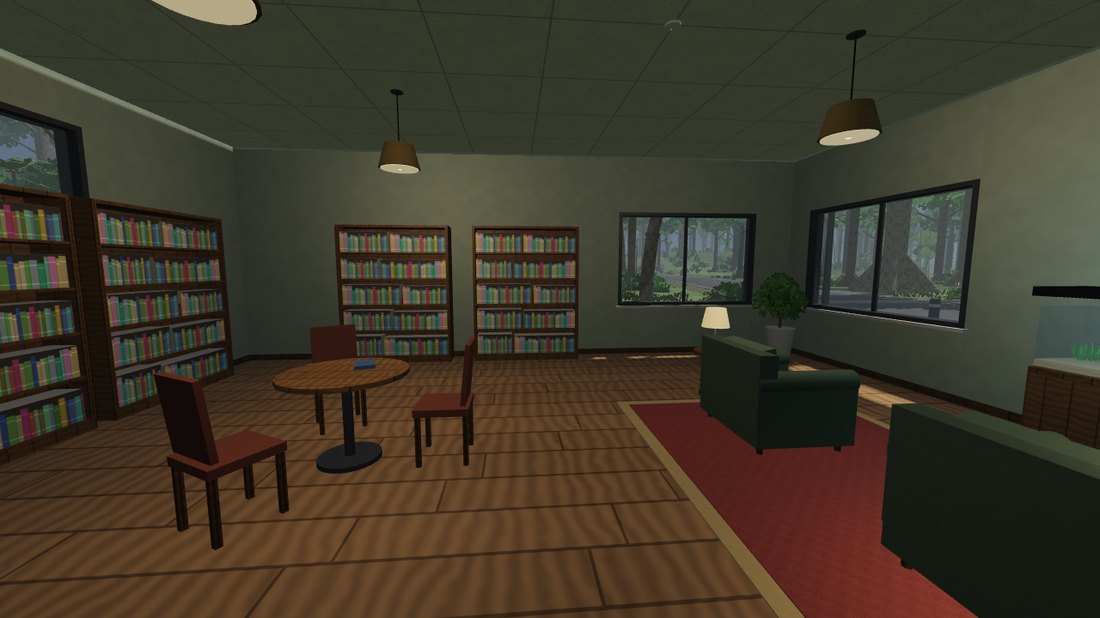
\includegraphics[width=\linewidth]{library_day}\caption{Library}\end{subfigure}
\begin{subfigure}{0.49\linewidth}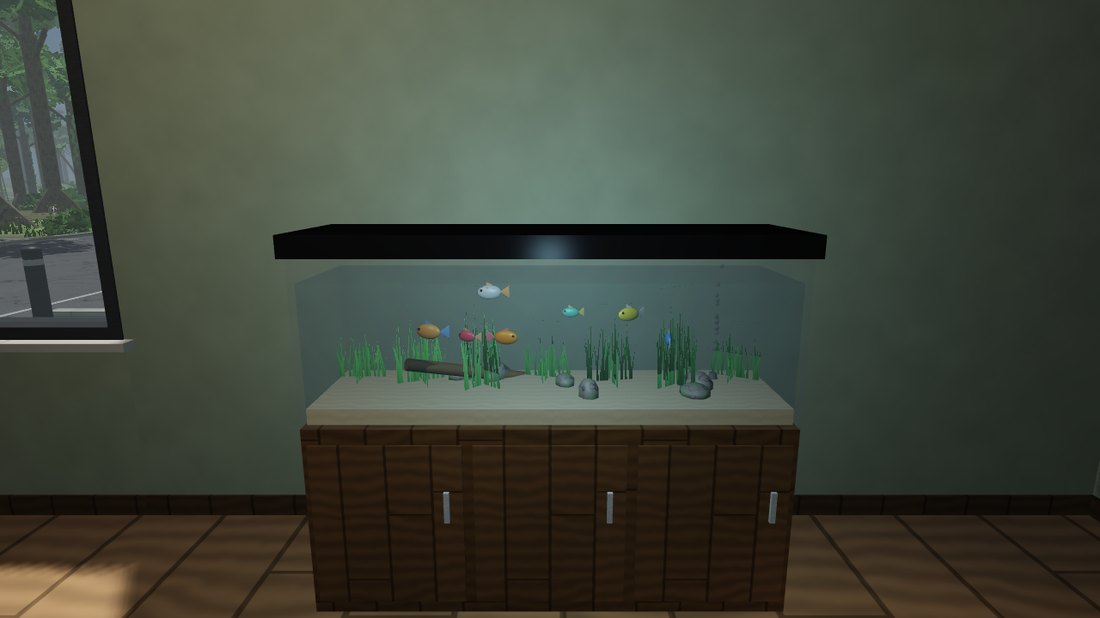
\includegraphics[width=\linewidth]{aquarium}\caption{Aquarium in the library}\end{subfigure}
\caption{The ATM room, the coffee counter and the library.}\label{fig:rooms}
\end{figure}
\begin{figure}[H]
\centering
\begin{subfigure}{0.49\linewidth}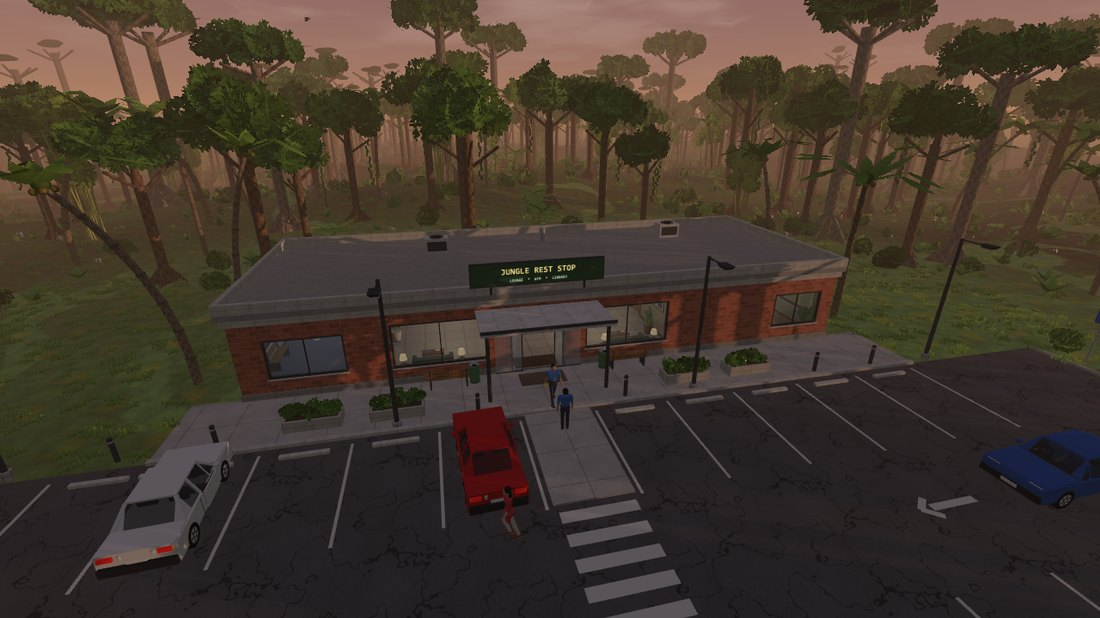
\includegraphics[width=\linewidth]{ext_sunrise}\caption{Sunrise 6:18}\end{subfigure}
\begin{subfigure}{0.49\linewidth}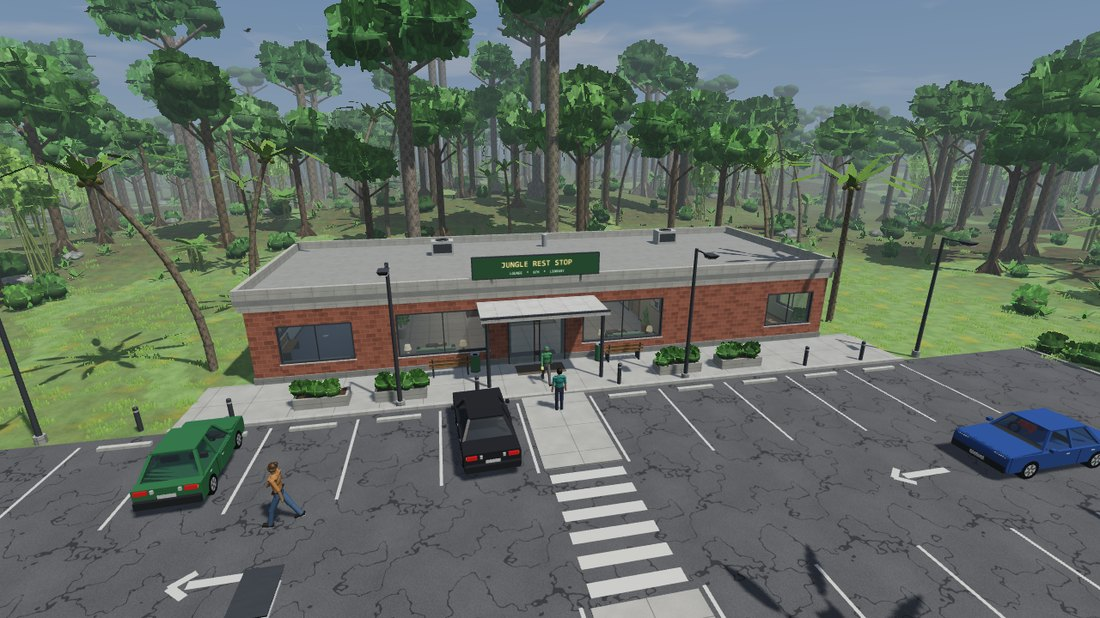
\includegraphics[width=\linewidth]{ext_day}\caption{Day 10:30}\end{subfigure}
\begin{subfigure}{0.49\linewidth}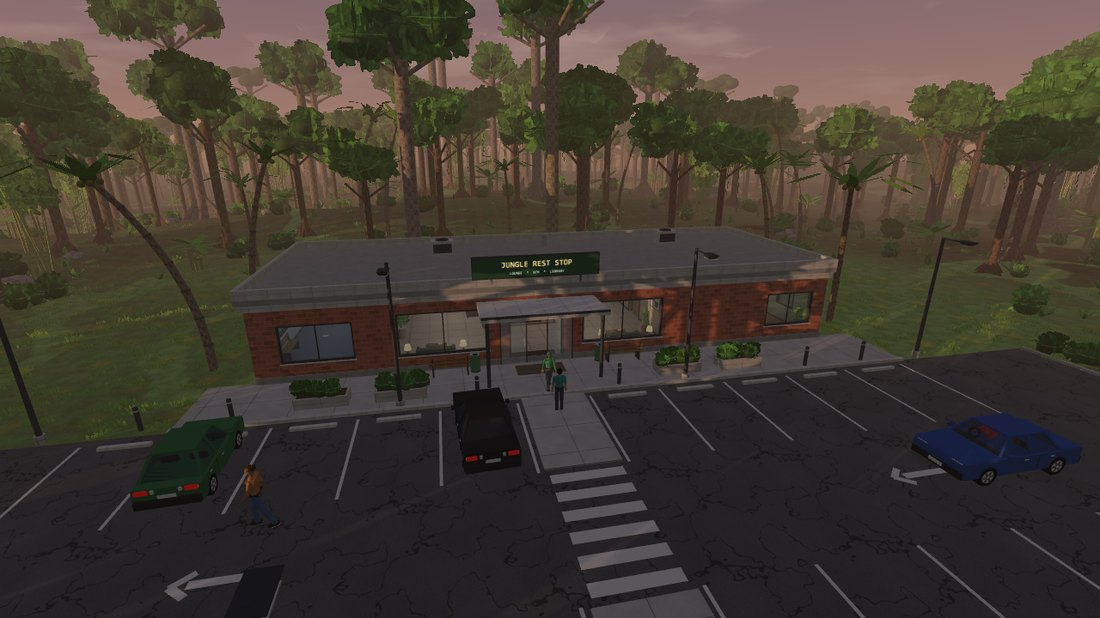
\includegraphics[width=\linewidth]{ext_sunset}\caption{Sunset 17:36}\end{subfigure}
\begin{subfigure}{0.49\linewidth}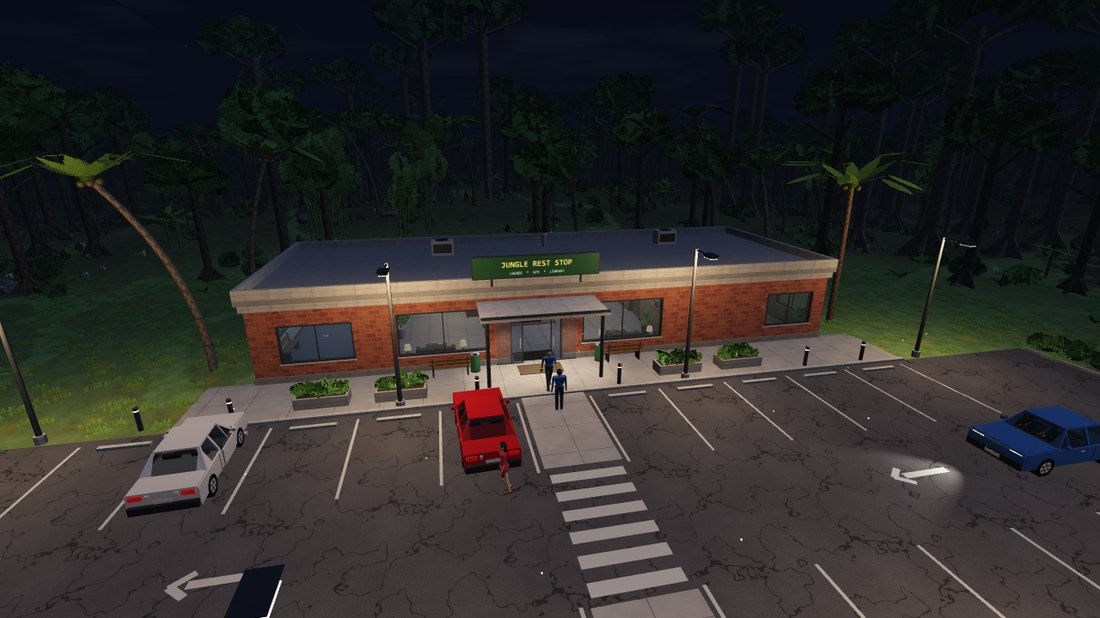
\includegraphics[width=\linewidth]{ext_night}\caption{Night 21:00}\end{subfigure}
\caption{The same view at four times of day.}\label{fig:daytimes}
\end{figure}

% =============================================================================
\section{Tools and Environment}
\begin{table}[H]
\centering\small
\begin{tabular}{@{}ll@{}}
\toprule
Item & Used \\ \midrule
Language & C++17 (MinGW-w64 / MSYS2 \texttt{g++}) \\
Graphics API & OpenGL 3.3 Core profile, GLSL 330 \\
Window / input & GLFW 3 \\
OpenGL loader & GLAD 2 \\
Text & Windows GDI renders one font atlas at start-up (Consolas) \\
Sound & Windows \texttt{waveOut} (winmm); 14 short CC0 (public domain) recordings \\
Assets & no models, no images: all meshes and textures are generated in code; only the sounds are files \\
Test PC & Intel Core i5-1135G7, Intel Iris Xe (integrated GPU), 1280$\times$720 window, 4$\times$MSAA \\
\bottomrule
\end{tabular}
\end{table}

% =============================================================================
\section{Controls}\label{sec:controls}
The scene is controlled with the keyboard and the mouse. Pressing \textbf{H} shows the same list inside
the program (\Cref{fig:help}).
\begin{table}[H]
\centering\small
\caption{Keyboard and mouse controls}\label{tab:controls}
\begin{tabularx}{\linewidth}{@{}P{3.3cm}X P{3.0cm}X@{}}
\toprule
Key & Action & Key & Action \\ \midrule
W A S D & walk & Shift & run \\
Mouse & look around & Space & jump \\
E / left click & use the part under the crosshair & V & camera: first person, third person, free \\
Mouse wheel, + / -- & change the field of view & Alt & free the mouse to click the on-screen buttons \\
B & Basic / Enhanced rendering & T, G, F & textures, shadows, fog on / off \\
N & switch day / night & [ \ ] & slower / faster time \\
M & pause the clock & R & roof cut-away view \\
F1 -- F4 & lounge, spot, room and outdoor lights & K & call a visitor car \\
L & frame cap 30 / 60 FPS & O & sound on / off \\
F12 & save a screenshot & H, Esc & help screen, quit \\
\bottomrule
\end{tabularx}
\end{table}
\begin{figure}[H]\centering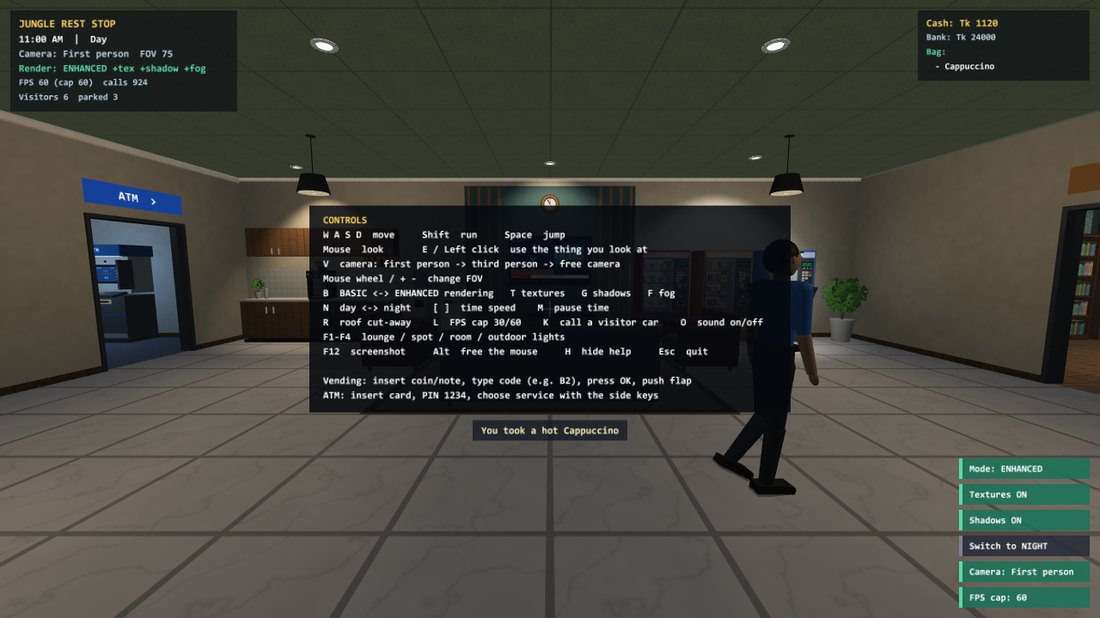
\includegraphics[width=0.8\linewidth]{help_screen}\caption{The help screen (H), with the status panel (top left), the wallet and the bag (top right) and the clickable buttons (bottom right).}\label{fig:help}\end{figure}
